\documentclass[a4paper, 11pt]{article}
%\usepackage[UTF8]{ctex}
%\usepackage{fontspec}
%\setmainfont{Fira Code}	% 设置全局英文字体(代码)
%\setCJKmainfont{宋体} 	% 设置全局中文字体

%\usepackage{fancyhdr} 	% 页眉页脚
%\usepackage{lastpage} 	% 获得总页数

% 插入图片的宏包
\usepackage{subfigure}
\usepackage{graphicx} 	% 插入图片的宏包
\graphicspath{{pic/}} 	% 在于.tex同级的目录下创建名为pic的文件夹,存放图片

% 超链接
\usepackage[colorlinks,linkcolor=red]{hyperref}

% 防止右边界越界(取消首段缩进?)
\raggedright 		  
% 首行缩进两格
\usepackage{indentfirst}
\setlength{\parindent}{2em}
% 页边距
\usepackage{geometry}
\geometry{a4paper,left=3cm,right=3cm,top=2cm,bottom=2cm}

\usepackage{amssymb} 	%不等号 等符号
\usepackage{amsmath} 	% 这是用于数学公式编辑的宏包
\usepackage{listings} 	% 用于插入代码块的宏包
\usepackage{xcolor}
\usepackage{color}
\usepackage{longtable}

\title{	
\normalfont \normalsize
\textsc{School of Data and Computer Science, Sun Yat-sen University} \\ [25pt] %textsc small capital letters
\rule{\textwidth}{0.5pt} \\[0.4cm] % Thin top horizontal rule
\huge DQN Breakout \\ % The assignment title
\rule{\textwidth}{2pt} \\[0.5cm] % Thick bottom horizontal rule
\author{18340047 Xiaolong Guo, 18308045 Zhengyang Gu}
\date{\normalsize\today}
}

\begin{document}
\maketitle
\tableofcontents
\newpage
\definecolor{mygreen}{rgb}{0,0.6,0}
\definecolor{mygray}{rgb}{0.5,0.5,0.5}
\definecolor{mymauve}{rgb}{0.58,0,0.82}
% 定义一些自用的颜色深度
% 设置显示代码颜色
\lstset{
      backgroundcolor=\color{white},  % 代码块背景颜色
      %basicstyle=\footnotesize \fontspec{Fira Code},       % 用于代码的前端显示
      breakatwhitespace=false,        % 若设置中断则发现在空白区
      breaklines=true,                % 设置自动断行
      captionpos=bl,                  % 设置标题位置为底端显示
      commentstyle=\color{mygreen},   % 注释风格颜色
      deletekeywords={...},           % 用于删除某关键字
      escapeinside={\%*}{*)},
      extendedchars=true,
      frame=single,                   % 在代码块区域增加边框
      keepspaces=true,
      keywordstyle=\color{blue},      % 关键词的颜色
      %language=C++               	% 要在代码块插入的代码类型
      morekeywords={*,...},           % if you want to add more keywords to the set
      numbers=left,
      numbersep=5pt,
      numberstyle=\tiny\color{mygray},% 行号字体的颜色
      rulecolor=\color{black},
      showspaces=false,
      showstringspaces=false,
      showtabs=false,
      stepnumber=1,                   % the step between two line-numbers
      stringstyle=\color{red},        % 双引号内的颜色
      tabsize=2,
}
\section{Breakout}
\subsection{Introduction}
In a Breakout game:
\begin{itemize}\setlength{\itemsep}{-\itemsep}
      \item A player is given a paddle that it can move horizontally
      \item At the beginning of each turn, a ball drops down automatically from somewhere in the screen
      \item The paddle can be used to bounce back the ball
      \item There are layers of bricks in the upper part of the screen
      \item The player is awarded to destroy as many bricks as possible by hitting the bricks with the bouncy ball
      \item The player is given 5 turns in each game
\end{itemize}

\section{Explanation of the original implementation}
We made some comments in the codes,
which were our understanding of each part of the codes.
\subsection{utils\_types.py}
There is no original static type checking in python,
which will brought us some unpredictable errors.
However, it can be acheived through the \emph{typing} module,
as shown below.
\begin{lstlisting}[language=python]
def __init__(self, device: TorchDevice) -> None:
  pass
\end{lstlisting}
This example specifies the type of parameters and return.
However, if a variable is specified as the \emph{Any} type,
python won't perform a static type checking on it.

The function of this file is as the comments said.
It's not for static type checking,
but it acts as hints for human only.
\begin{lstlisting}[language=python]
"""
Aliases created in this module are useless for static type checking, instead,
they act as hints for human only
"""
\end{lstlisting}


\subsection{utils\_model.py}
This file defines the \emph{DQN} class
which is the network used by the dqn algorithm.
\begin{itemize}\setlength{\itemsep}{-\itemsep}
      \item The \emph{forward} method:
            The input is the state whose length is 4.
            And the output is the evaluation of the state
            calculated by the forward algorithm.
            This method can be called in the form of
            \emph{model\_var(x)} which is equavalent to \emph{model\_var.forward(x)}.
      \item The \emph{init\_weights} method:
            The function of this method is to initiate the weights of the network.
\end{itemize}

\subsection{utils\_model.py}
The difference between \emph{state} and \emph{folded\_state}
needs to be clarified at first.
\begin{itemize}\setlength{\itemsep}{-\itemsep}
      \item The \emph{state} is a variable of length 4,
            while the \emph{folded\_state} is a variable of length 5.
      \item The \emph{state} denotes s single state,
            while the \emph{folded\_state} represents the folded form
            of two continuous states,
            of which [:4] is the current state and [1:] is the next state.
\end{itemize}

This file defines the \emph{ReplayMemory} class
whcih is the replay memory used by dqn algorithm.
\begin{itemize}\setlength{\itemsep}{-\itemsep}
      \item The \emph{push} method:
            The input is \emph{(folded\_state, action, reward, done)}
            in which \emph{done} is a boolean
            that denotes whether the game is over.
            The method stores these variables in the memory.
      \item The \emph{sample} method:
            The input is the size of batch.
            And the method randomly samples a batch
            in which \emph{folded\_state} is restored to
            \emph{state} and \emph{next}.
\end{itemize}

\subsection{utils\_drl.py}
This file implements the dqn algorithm
through defining the \emph{Agent} class.
\begin{itemize}\setlength{\itemsep}{-\itemsep}
      \item The \emph{run} method:
            This method chooses an action by applying
            $\epsilon$-greedy algorithm.
      \item The \emph{learn} method:
            This method trains the policy network using nature dqn algorithm.
      \item The \emph{sync} method:
            This method copies the weights
            from policy network to target network.
      \item The \emph{save} method:
            This method saves the state dict of the policy network.
\end{itemize}

\subsection{utils\_env.py}
This file implements the breakout's environment \emph{MyEnv}
using atari environment provided by deepmind.
\begin{itemize}\setlength{\itemsep}{-\itemsep}
      \item The \emph{reset} method:
            This method resets and
            initializes the underlying gym environment.
            It takes \emph{render} as the input,
            which is used to decide whether
            the environment renders images.
      \item The \emph{step} method
            This method forwards an action to the environment
            and returns the newest observation, the reward,
            and an bool value indicating whether the
            episode is terminated.
      \item The \emph{evaluate} method:
            This method uses the given agent to run the game for
            a few episodes and returns the average reward
            and the captured frames.
            It takes \emph{(obs\_queue, agent, num\_episode, render)}
            as the input.
            The \emph{obs\_queue} is an obervation queue of length 5,
            which can be converted into \emph{folded\_state}.
            The \emph{num\_episode} specifies the number of episodes
            that the game will be run for.
\end{itemize}

\subsection{main.py}
This file is the entrance of all of the codes.
It defines some hyperparameters of the model
and combines all codes together.
\begin{itemize}\setlength{\itemsep}{-\itemsep}
      \item \emph{MAX\_STEPS}:
            This hyperparameter denotes the max steps
            the environment runs.
            Every step the \emph{run} method is called once
            to get the action generated by the model.
            And the \emph{step} method is called once
            and takes the action as input.
            And the \emph{push} method is called once
            to update the memory.
      \item \emph{WARM\_STEPS}
            This hyperparameter denotes the steps
            that the environment runs before training.
      \item \emph{POLICY\_UPDATE}
            This hyperparameter denotes the frequency
            of the update of policy network.
            Every time the policy network updates,
            the \emph{learn} method is called once.
      \item \emph{TARGET\_UPDATE}
            This hyperparameter denotes the frequency
            of the update of target network.
            Every time the target network updates,
            the \emph{sync} method is called once.
      \item \emph{EVALUATE\_FREQ}
            This hyperparameter denotes the frequency
            of the evaluation.
            Every time the the evaluation is being done,
            the \emph{evaluate} method is called once
            to get the average reward, and to get frames depending on
            whether \emph{RENDER} is True.
            And those data will be stored in disk as the form of files.
\end{itemize}

\section{research}
\subsection{Abstract}
We tried to improve the given implementation \cite{ref1} of Nature-DQN for Breakout game in four ways: 1. change the Nature-DQN to a Double-DQN 2. use the Priortized Experience Replay 3. change the model to a Dueling DQN 4. add stable reward to the network to stablize the movement. We successfully implement the four methods and their combinations, which were open-sourced on github \cite{ref2}. With ablation studies, we conclude that both our improvement 3 and 4 are useful for the breakout game, while 1 and 2 are not, which is similar to the result of Rainbow DQN research \cite{ref7}
\subsection{Related Works}
\subsubsection{Double DQN}
In Nature DQN, non-terminated states' s $Q$
value can be calculated by
$$y_j=R_j+\gamma\mathop{max}_{a'}Q'(\phi(S_j'),A_j',w')$$
while in Double DQN, the value is calculated via
$$y_j=R_j+\gamma Q'(\phi(S_j'),arg\ \mathop{max}_{a'}Q(\phi(S_j'),a,w),w')$$
.The difference between them is that the Nature DQN directly
uses the max Q value of next state estimated by target network,
while the Double DQN first find the best action using
the policy network, and then use the target network to calculate
the Q value of next state after doing that action.
This helps to avoid overfitting\cite{ref3}.
\subsubsection{Prioritized Experience Replay}
Prioritized DQN \cite{ref4} adopts PER(Prioritized Experience Replay) to speed up
the training process.
The PER introduce a kind of priority mechanism, which prefers those that
have bigger TD-error since the bigger TD-error means the bigger gap between
estimated Q value and goal.
In addition, a sumtree needs to be implemented to store the priority to
have a better perfomance.
\subsubsection{Dueling DQN}
Dueling DQN \cite{ref6} devides the model into two parts, one of which is state
function which estimates the value of states, the other of which is
advantage function which estimates the value of actions.
$$Q(s,a,w,\alpha,\beta)=V(s,w,\alpha)+A(s,a,w,\beta)$$
Additionally, centralization has to be done to ensure that the sum of
the Q value with the same states and differnent actions has nothing to do
with the second term of the formula, but it just depends on
the state function.
$$Q(s,a,w,\alpha,\beta)=V(s,w,\alpha)+(A(s,a,w,\beta)
      -\frac{1}{|\mathcal{A}|}\sum_{a'\in\mathcal{A}}A(s,a',w,\beta))$$
\subsection{Our Implementation}
\subsubsection{Double DQN}
We simply change the network form Nature DQN to Double DQN as follow.
\begin{lstlisting}[language={python}]
	values_next = self.__target(next_batch.float()).gather(
            1, self.__policy(next_batch.float()).max(1).indices.unsqueeze(1)).detach()
	\end{lstlisting}
\subsubsection{Boost the training speed}
We use PER to speed up the training. In our implementation, we use an open source implementation of PER. With DDQN implemented and PER peovided, we fix our code according to the pseudocode provided by \cite{ref4}, which is shown in figure \ref{PER}.

First, we adjust the experience in PER as the form we already have. Second, we replace the origin memory class' instantiation and method calls with PER's. Finally, we add priority update and importance sampling like line 11 to 13 in figure \ref{PER}.

Thea final step is shown bellow, please refer to our code for more details.
\begin{lstlisting}[language={python}]
		td_error = (expected - values).detach()
    memory.update_priority(rank_e_id, td_error.cpu().numpy())

    values = values.mul(w)
    expected = expected.mul(w)
    loss = F.smooth_l1_loss(values, expected)
	\end{lstlisting}
\begin{figure}[ht]
      \centering
      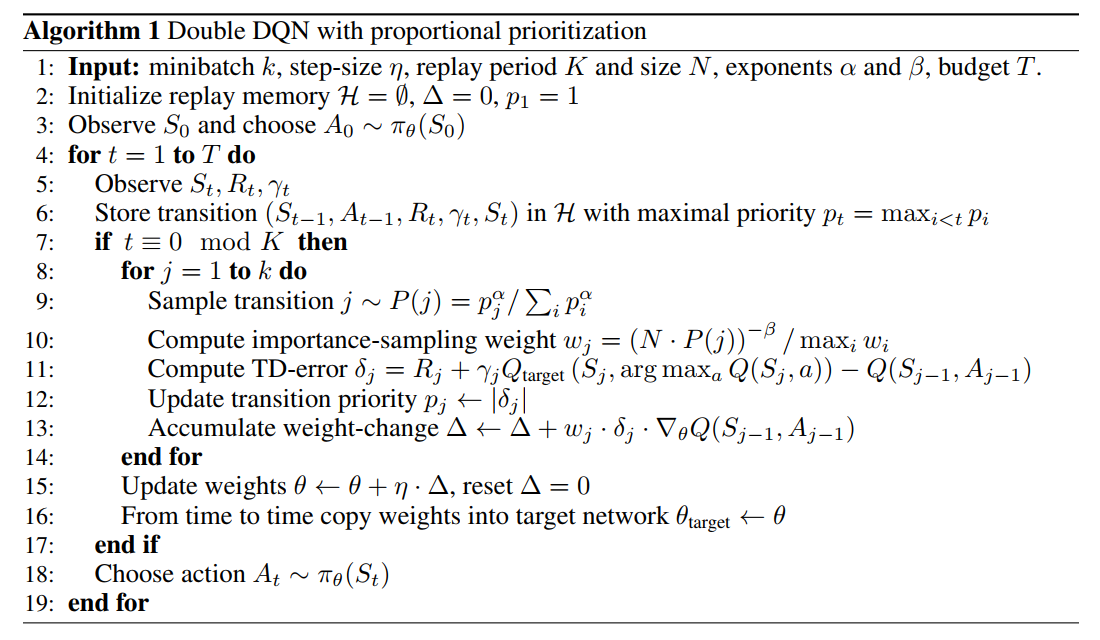
\includegraphics[width = 0.8 \textwidth]{per}
      \caption{Prioritized experience replay DQN pseudocode from \cite{ref4}}
      \label{PER}
\end{figure}
\subsubsection{Improve the performance}
We use Dueling DQN to improve the performance. What we need to do is changing the network model for value function for approximation as follow, which can be visualized as figure \ref{DUEL}
\begin{lstlisting}[language={python}]
class DQN(nn.Module):  # duel dqn

    def __init__(self, action_dim, device):
        super(DQN, self).__init__()
        self.__conv1 = nn.Conv2d(4, 32, kernel_size=8, stride=4, bias=False)
        self.__conv2 = nn.Conv2d(32, 64, kernel_size=4, stride=2, bias=False)
        self.__conv3 = nn.Conv2d(64, 64, kernel_size=3, stride=1, bias=False)
        self.__fc1 = nn.Linear(64 * 7 * 7, 512)
        self.__fc2 = nn.Linear(512, action_dim) 
        self.__fc1a = nn.Linear(64 * 7 * 7, 512)  
        self.__fc2a = nn.Linear(512, 1) 
        self.__device = device

    def forward(self, x):
        x = x / 255.
        x = F.relu(self.__conv1(x))
        x = F.relu(self.__conv2(x))
        x = F.relu(self.__conv3(x))
        advantagex = F.relu(self.__fc1(x.view(x.size(0), -1)))
        advantage = self.__fc2(advantagex)
        valuex = F.relu(self.__fc1a(x.view(x.size(0), -1)))
        value = self.__fc2a(valuex)
        return value + (advantage - advantage.mean(1, keepdim=True)) 
	\end{lstlisting}
\begin{figure}[ht]
      \centering
      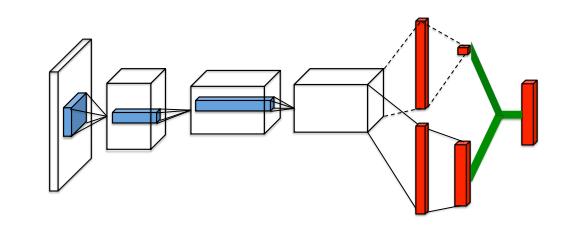
\includegraphics[width = 0.8 \textwidth]{dueling}
      \caption{Dueling network architecture from \cite{ref6}.}
      \label{DUEL}
\end{figure}
\subsubsection{Stablize the movement}
To satble the movement of paddle in the Breakout game, we have two ideas, one is policy based and the other is model based:
\begin{itemize}
      \item policy-based: since the policy is $\epsilon$-greedy, we can give a much larger probability for actions that can stablized the movement, like no-op actions or actions that keep a certain moving direction.
      \item model-based: simply give a extra reward to actions that help the stable.
\end{itemize}
It's much easier to implement the model-based method, so we chose it and implemented it as follow.
\begin{lstlisting}[language={python}]
reward_batch[action_batch == 0] += 0.1  # stable reward
	\end{lstlisting}
The method may destroy the model-free quality of DRL, for it requires the network to konw what actions are no-ops. But it's still intuitive and has the ability to represent the cost of action in real word or energy cost for human players.
\subsection{Experiment}
\subsubsection{Priortized Dueling Double DQN}
\begin{figure}[htbp]
      \centering
      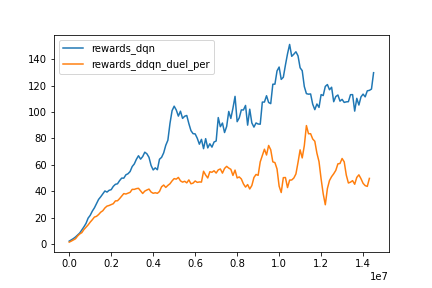
\includegraphics[width = 0.6 \textwidth]{01}
      \caption{the reward curve of PDD-DQN and Nature DQN baseline in Breakout game. Every curve is smoothed with a moving
            average of 10 to improve readability}\label{res1}
\end{figure}
We compose all the improvement above except the stable component together as a Priortized Dueling Double DQN(PDD-DQN), and gain performance shown by figure \ref{res1}. Our PDD-DQN appears to work even woser than Nature DQN in the Breakout game. So we need to do ablation studies to find out what's the reason.
\subsubsection{ablation studies}
\begin{figure}[htbp]
      \centering
      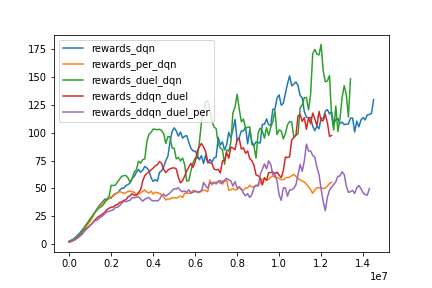
\includegraphics[width = 0.6 \textwidth]{02}
      \caption{ablation studies on components of SPDD-DQN. With only the Dueling component, it works better than baseline. Once adding other components like Double DQN and Prioritized DQN, it's performance decrease lower than baseline. Every curve is smoothed with a moving average of 10.}\label{res2}
\end{figure}
\begin{figure}[htbp]
      \centering
      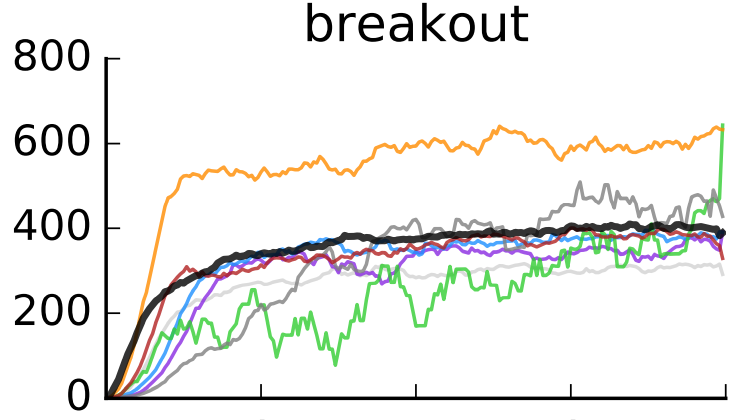
\includegraphics[width = 0.5 \textwidth]{11}
      
\includegraphics[width = 0.5 \textwidth]{12}
      \caption{results on Breakout game  of the Rainbow DQN research \cite{ref7}. Even Rainbow DQN doesn't work much better than Nature DQN on this game. Double DQN and Prioritized DQN are shown to have lower performance than baseline before the reward reaches 200.}\label{res3}
\end{figure}
\begin{figure}[htbp]
      \centering
      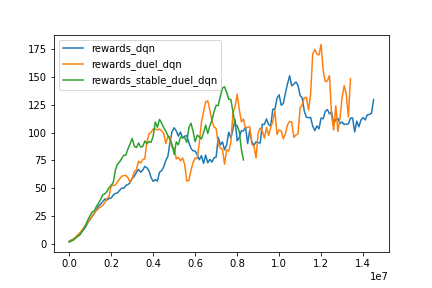
\includegraphics[width = 0.6 \textwidth]{03}
      \caption{learning curve of Stable Dueling DQN, with Dueling DQN and baseline compared. With a stable component, Stable Dueling DQN keeps and improves the advantage of Dueling DQN to the baseline.}\label{res4}
\end{figure}
The result of ablation studies was show in figure \ref{res2}. We found that Dueling DQN has higher performance than Nature DQN in Breakout game, while Double DQN and Prioritized DQN have lower.
\subsubsection{compared with others}
To validate our result, we compare it with Rainbow DQN research \cite{ref7}, whose result in Breakout game is shown in figure \ref{res3}. We found that in Breakout game, what the research of Rainbow DQN gains is similar to ours, where the performance of DQN is better than Double DQN and Prioritized DQN before the reward reaches 200.
\subsubsection{stable component}
We plot the learning curve of Stable Dueling DQN, with baseline and Dueling DQN compared, which is shown in figure \ref{res4}. We found that the stable component didn't destroy the advantage of Dueling DQN, but improve it a little.

To see how much the Stable Dueling DQN stablize the paddle, we pick the models of same epoch in it and Dueling DQN and compare the playing video generated by the models, which can be watch in attachment. We found the the stable component can stablize the movement, to a certain extent.
\subsection{Conclusions}
We implemented a Stable Prioritized Dueling Double DQN(SPDD-DQN) for the Breakout game and found the stable component and dueling component of the network can effectively improve the performance, while the Prioritized component and Double DQN component do not work well, which is similar to the result on Breakout game of the Rainbow DQN research \cite{ref7}.

Future work may include the experiment with more running epochs and the experiment on other games.
\subsection{Acknowledgments}
Thanks to the authors of open source code \cite{ref5}.

Thanks to the baseline result shared by 18340043.

Thanks to the HPC provided by SYSU.

Authorship matrix is as follow.
\begin{center}
      \begin{tabular}{cccc}
            \hline
            Member       & Ideas(\%) & Coding(\%) & Writing(\%) \\
            \hline
            Xiaolong Guo & 60        & 60         & 40          \\
            Zhengyang Gu & 40        & 40         & 60          \\
            \hline
      \end{tabular}
\end{center}
\begin{thebibliography}{99}
      \bibitem{ref1} https://github.com/lukeluocn/dqn-breakout
      \bibitem{ref2} https://github.com/guzy0324/dqn-breakout
      \bibitem{ref3} van Hasselt, H.; Guez, A.; and Silver, D. 2016. Deep reinforcement learning with double Q-learning. In Proc. of AAAI, 2094–2100.
      \bibitem{ref4} Schaul, T.; Quan, J.; Antonoglou, I.; and Silver, D. 2015.
      Prioritized experience replay. In Proc. of ICLR.
      \bibitem{ref5} https://github.com/Damcy/prioritized-experience-replay
      \bibitem{ref6} Wang, Z.; Schaul, T.; Hessel, M.; van Hasselt, H.; Lanctot,
      M.; and de Freitas, N. 2016. Dueling network architectures for deep reinforcement learning. In Proceedings of The
      33rd International Conference on Machine Learning, 1995–2003.
      \bibitem{ref7}  van Hasselt, H.; Hessel, M.; and Silver, D. 2017. Rainbow: Combining Improvements in Deep Reinforcement Learning.
\end{thebibliography}




\end{document}





